\chapter{Grundlagen}
\label{chap:grundlagen}

Diese Kapitel gibt einen Überblick über die Grundlagen, die für das Verständnis dieser Arbeit notwendig sind. Zunächst wird der Begriff \textit{Instant-Messaging} definiert und es werden die beiden grundlegenden Arten von Instant-Messaging-Protokollen, zentralisierte und dezentrale, beschrieben. Darauf folgt eine kurze Vorstellung von bereits existierenden Instant-Messaging-Protokollen, die als Grundlage für die Entwicklung eines eigenen Protokolls dienen. Danach wird die Peer-to-Peer-Technologie beschrieben, mit deren Hilfe die Kommunikation zwischen den Benutzern eines dezentralen Instant-Messaging-Protokolls stattfindet. Anschließend werden Methoden zur Sicherung der Kommunikation  beschrieben, die in der Regel in Instant-Messaging-Protokollen verwendet werden. Abschließend wird die Blockchain-Technologie definiert und ihre Funktionsweise beschrieben.

\section{Instant Messaging}
% Was ist Instant Messaging?
% Wofür wird es verwendet?
% Welche Anwendungen gibt es? (WhatsApp, Signal, Telegram, Threema, etc.) -> die meisten sind zentralisiert
% Welche Probleme gibt es bei zentralisierten Anwendungen?
% Client-Server-Architektur und Peer to Peer als Überleitung zur nächsten Sektion verwenden


Instant Messaging bezeichnet eine Form der Kommunikation, bei der Nachrichten in Echtzeit zwischen zwei oder mehreren Personen über das Internet ausgetauscht werden können \Parencite[S. 69]{nist_mobileDeviceForensics}. Diese Form der digitalen Kommunikation ermöglicht es Nutzern, sofortige Nachrichten, Bilder und andere Mediendateien auszutauschen. Instant Messaging-Dienste umfassen eine Vielzahl von Plattformen und Anwendungen, die es Benutzern ermöglichen, miteinander zu kommunizieren, sei es eins zu eins oder in Gruppenchats. Instant-Messaging-Dienste reichen von plattformübergreifenden Anwendungen wie \textit{WhatsApp}, \textit{Signal} und \textit{Telegram} bis hin zu spezialisierten Unternehmenslösungen wie \textit{Slack} oder \textit{Microsoft Teams}. Die Vielfalt an Funktionen in Instant-Messaging-Plattformen ist groß. Neben einfachen Textnachrichten können Benutzer zum Beispiel mit der App \textit{WhatsApp} Emojis, Aufkleber, GIFs und Sprachnachrichten teilen, was die Kommunikation dynamisch und ausdrucksstark gestaltet \Parencite{whatsapp_funktionen}. Gruppenchats ermöglichen es mehreren Personen, in einer einzigen Unterhaltung zusammenzukommen, was die Zusammenarbeit, soziale Interaktion und Informationsverbreitung erleichtert.
Sicherheit und Datenschutz sind in der Welt des Instant Messaging von entscheidender Bedeutung. Verschlüsselungstechnologien werden verwendet, um die Vertraulichkeit der Nachrichten zu gewährleisten und die Privatsphäre der Nutzer zu schützen. Die Authentifizierung von Benutzern, End-to-End-Verschlüsselung und andere Sicherheitsmechanismen sind unerlässlich, um die Integrität der Kommunikation zu gewährleisten.

Instant Messaging-Anwendungen können auf verschiedene Arten strukturiert sein, wobei zwei Hauptansätze hervorstechen: die Client-Server-Architektur und das Peer-to-Peer-Modell.
Die Client-Server-Architektur ist bei vielen gängigen Instant Messaging-Diensten verbreitet. Hierbei fungiert ein zentraler Server als Vermittler zwischen den Benutzergeräten. Die Nachrichten werden von den Clients (den Benutzergeräten) an den Server gesendet, der sie dann an die Empfänger weiterleitet. Dieser Ansatz bietet eine einfache Verwaltung der Kommunikation, zentralisierte Datenverwaltung und ermöglicht Dienstleistungen wie das Offline-Speichern von Nachrichten.
Im Gegensatz dazu basiert das Peer-to-Peer-Modell (kurz: P2P) auf direkten Verbindungen zwischen den Benutzergeräten ohne die Notwendigkeit eines zentralen Servers. Jedes Gerät agiert sowohl als Client als auch als Server, wodurch die Kommunikation direkt zwischen den Teilnehmern stattfindet. Diese Struktur bietet potenzielle Vorteile in Bezug auf Datenschutz, da die Nachrichten nicht über einen zentralen Server geleitet werden müssen.
Beide Ansätze haben ihre eigenen Vor- und Nachteile. Die Client-Server-Architektur ermöglicht eine einfachere Verwaltung und Zuverlässigkeit, birgt jedoch potenzielle Datenschutzrisiken, da Daten zentralisiert gespeichert werden. Auf der anderen Seite bietet das Peer-to-Peer-Modell potenziell mehr Privatsphäre und Sicherheit, aber es könnte Schwierigkeiten bei der Skalierbarkeit und Verlässlichkeit geben, da es keine zentrale Instanz gibt, die die Kommunikation steuert. Die Wahl zwischen diesen Architekturen hängt von den spezifischen Anforderungen, Sicherheitsbedenken und dem Nutzungskontext der Instant Messaging-Anwendung ab.



\section{Peer-to-Peer-Technologie}
\label{subsec:peer_to_peer_technologie}
% #TODO: Funktion des Kademlia Protokolls nennen und erklären (vielleicht in Grundlagen)
% Im Kademlia-Protokoll sind vier Funktionen definiert, die für die Suche nach
% Knoten und Werten verwendet werden. Diese Funktionen sind \texttt{FIND\_NODE},
% \texttt{FIND\_VALUE}, \texttt{PING} und \texttt{STORE}. Die Funktionen
% \texttt{FIND\_NODE} und \texttt{FIND\_VALUE} werden verwendet, um nach Knoten
% oder Werten zu suchen. Die Funktion \texttt{PING} wird verwendet, um die
% Erreichbarkeit eines Knotens zu überprüfen. Die Funktion \texttt{STORE} wird
% verwendet, um einen Wert in einem Knoten zu speichern.

Peer-to-Peer-Technologien können in zwei Kategorien unterteilt werden: Peer-to-Peer-Anwendungen und Peer-to-Peer-Infrastrukturen. Die Kategorie der Peer-to-Peer-Anwen-\\dungen umfasst den Dienst der Inhaltsverteilung, bei dem die Teilnehmer Inhalte wie Musik, Videos oder andere Dateien direkt untereinander austauschen \Parencite[730-731]{Khatibi_StructuredUnstructuredP2P}. 

Daher werden viele Peer-to-Peer schnell mit Filesharing in Verbindung bringen, da diese Technologie in der Vergangenheit vor allem dafür genutzt wurde. Das bekannteste Beispiel ist das Filesharing-Netzwerk \textit{Napster}, das 1999 von Shawn \enquote{Napster} Fanning entwickelt wurde. \textit{Napster} war das erste weit verbreitete Filesharing-Netzwerk, das auf Peer-to-Peer-Technologie basierte. Es ermöglichte den Austausch von Musikdateien zwischen den Teilnehmern. Die Musikdateien wurden dabei auf den Computern der Teilnehmer gespeichert und konnten von anderen Teilnehmern heruntergeladen werden. Da diese Art des Datenaustauschs oftmals illegal war, wurde Napster 2001 aufgrund von Urheberrechtsverletzungen abgeschaltet \parencite[S. 55-57]{Mahlmann_P2PNetzwerke}.

Die Peer-to-Peer-Infrastruktur umfasst die Peer-to-Peer-Netzwerke, die für die Kommunikation zwischen den Teilnehmern verwendet werden \parencite[S. 730-731]{Khatibi_StructuredUnstructuredP2P}. Diese Arbeit konzentriert sich auf die Peer-to-Peer-Infrastruktur, die die Kommunikation zwischen den Teilnehmern ermöglichen soll.

Im Instant-Messaging-Bereich repräsentiert das Peer-to-Peer-Modell eine dezentrale Struktur, die dabei hilft, die Kommunikation zwischen den Teilnehmern zu ermöglichen. Im Gegensatz zum Client-Server-Ansatz, bei dem ein zentraler Server die Kommunikation zwischen den Teilnehmern steuert, ermöglicht das Peer-to-Peer-Netzwerk direkte Kommunikation zwischen den Teilnehmern. Beide Modelle bringen Vor- und Nachteile mit sich. Während das Client-Server-Modell eine zentrale Instanz erfordert, um die Kommunikation zu verwalten, ist das Peer-to-Peer-Netzwerk dezentralisiert und benötigt keine solche Instanz. Die Implementierung und Wartung eines Client-Server-Modells gestalten sich einfacher im Vergleich zu einem komplexeren und aufwendigeren Peer-to-Peer-Netzwerk. Das Client-Server-Modell ist weniger flexibel, da es von einer zentralen Instanz abhängt, während das Peer-to-Peer-Netzwerk aufgrund des Fehlens dieser Instanz flexibler ist. Skalierbarkeit ist ebenfalls ein Unterschied: Das Client-Server-Modell ist durch die Kapazität des Servers begrenzt, während das Peer-to-Peer-Netzwerk auf die Kapazität der Teilnehmer zurückgreift, was seine Skalierbarkeit verbessert. In Bezug auf Sicherheit ist das Client-Server-Modell weniger robust, da es auf eine zentrale Instanz angewiesen ist, während das Peer-to-Peer-Netzwerk, das ohne solche Abhängigkeit auskommt, als sicherer gilt \parencite[S. 6-8]{Mahlmann_P2PNetzwerke}.


\subsection{Typen von Peer-to-Peer-Netzwerken}

Nicht jedes Peer-to-Peer-Netzwerk ist gleich. Es gibt verschiedene Typen von Peer-to-Peer-Netzwerken, die sich in ihrer Struktur und Funktionsweise unterscheiden. Abbildung \ref{p2p_typen} zeigt die zwei Haupttypen von Peer-to-Peer-Netzwerken: unstrukturierte und strukturierte Netzwerke \parencite[S. 362-363]{Luntovskyy_ModRechnernetze}.

\begin{center}
    \captionsetup{type=figure}
    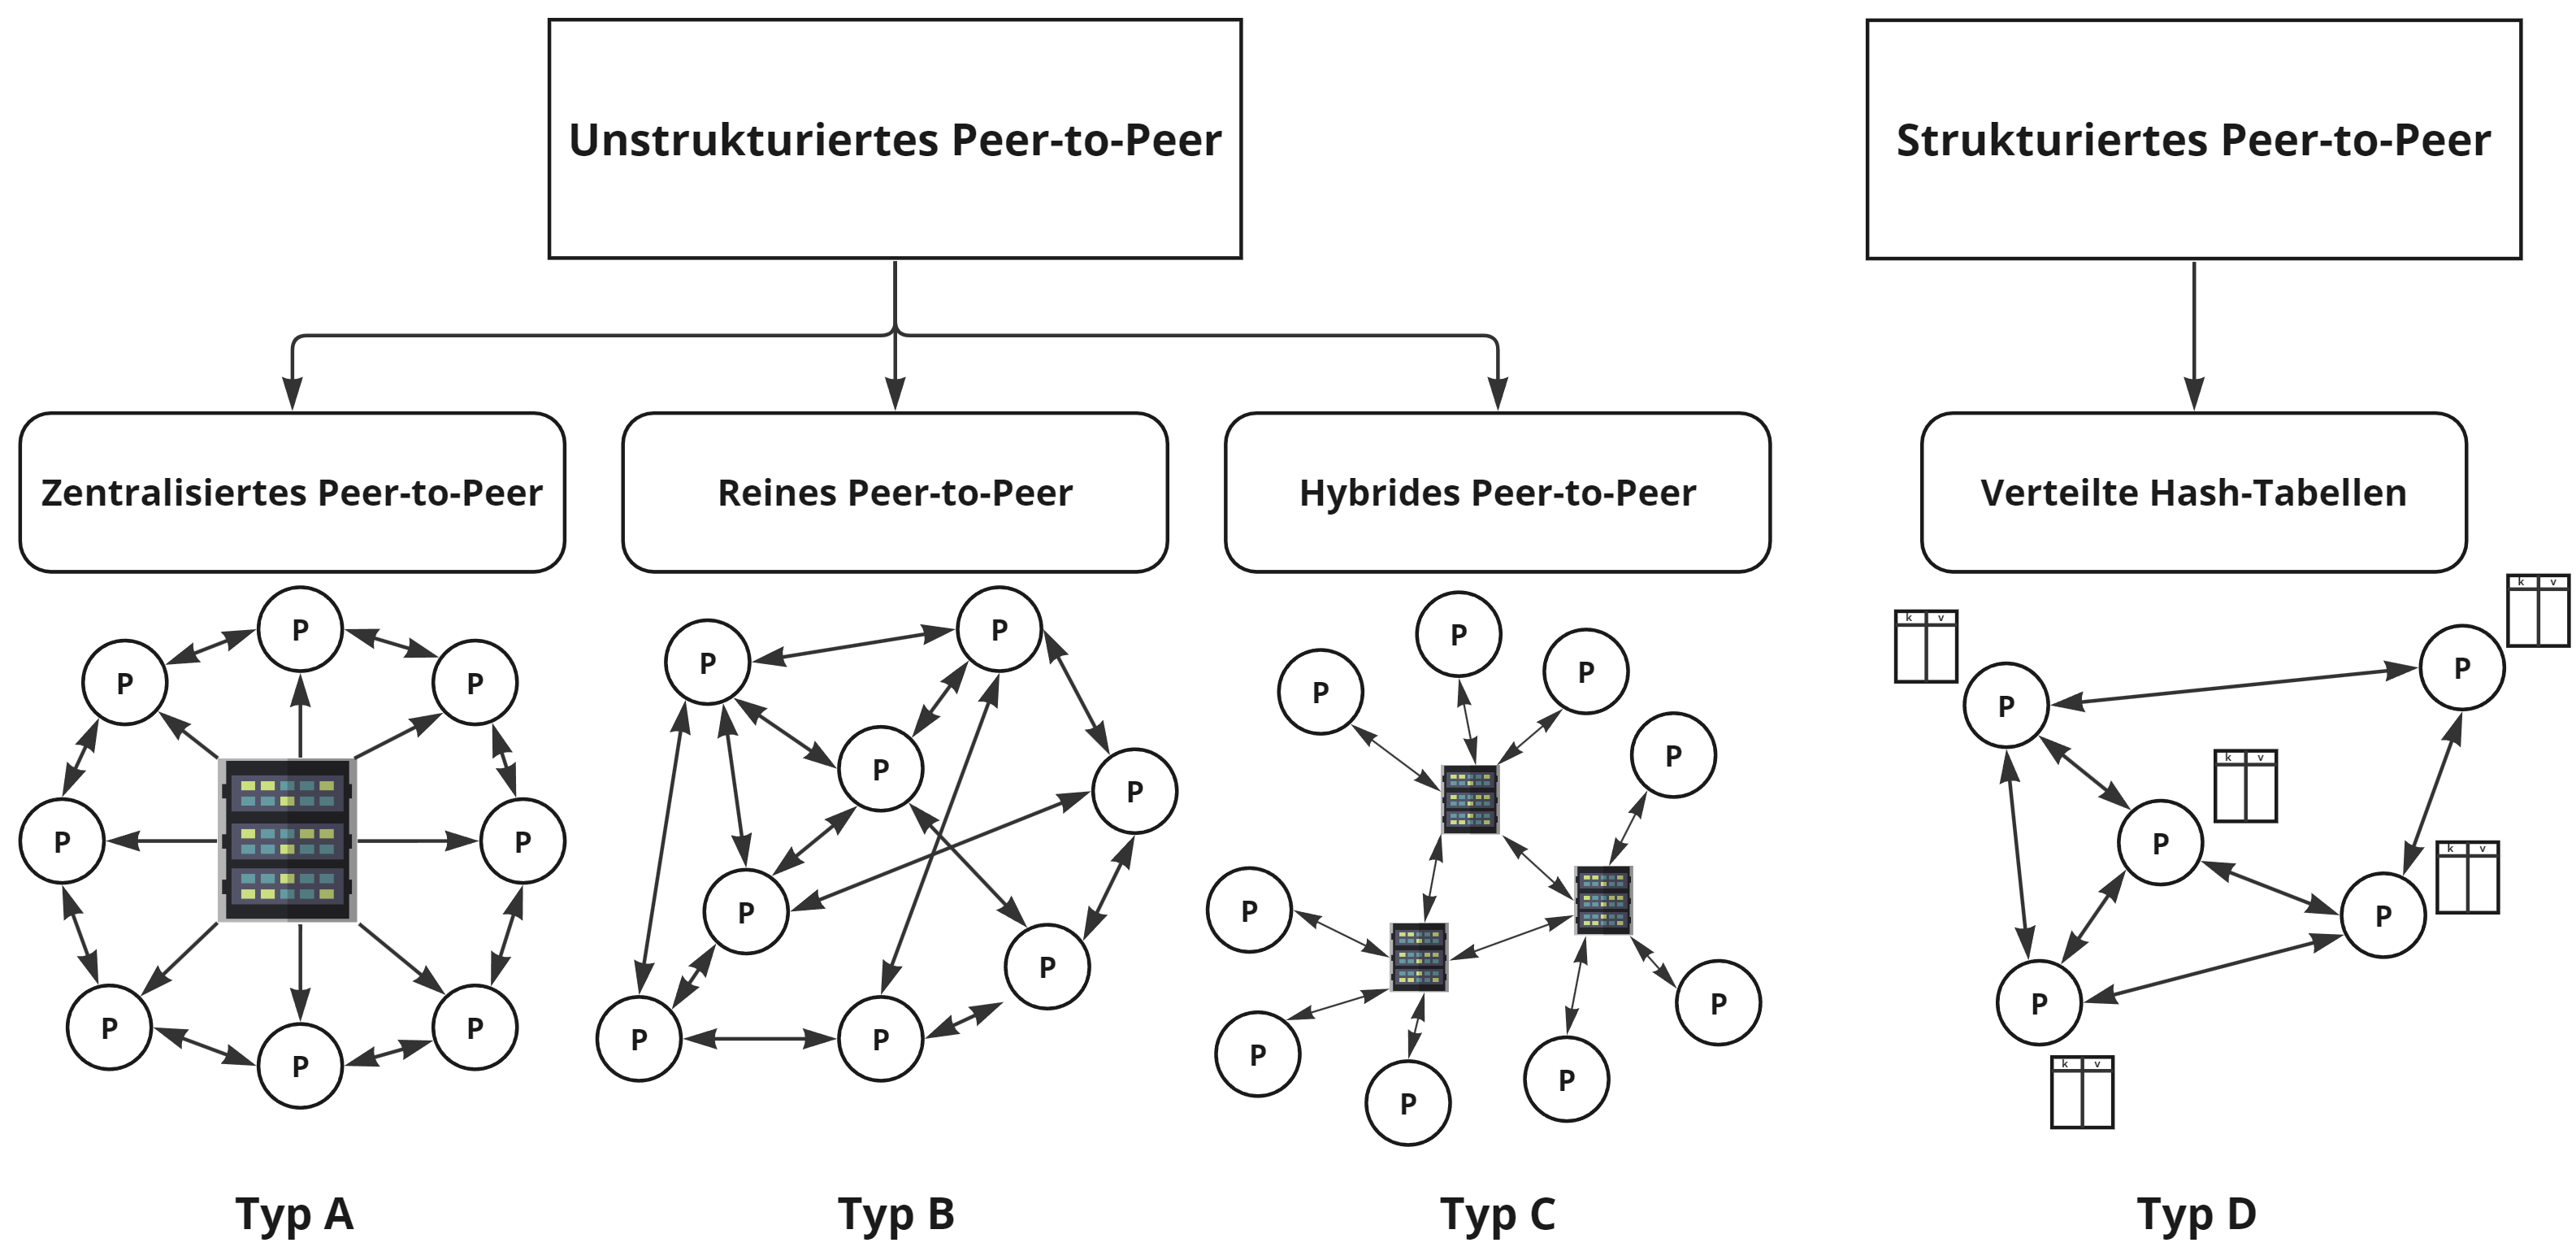
\includegraphics[width=1\linewidth]{images/p2p_typen.png}
    \captionof{figure}{Typen von Peer-to-Peer-Netzwerken, in Anlehnung an \cite[S. 363]{Luntovskyy_ModRechnernetze}}
    \label{p2p_typen}
\end{center}

\noindent Unstrukturierte und strukturierte Peer-to-Peer-Netzwerke sind unterschiedliche Ansätze zur Organisation von Knoten (engl. \textit{Nodes}) und Ressourcen in dezentralen Netzwerken.

Unstrukturierte Netzwerke sind charakterisiert durch ihre fehlende explizite Organisationsstruktur, was eine einfache Konnektivität ermöglicht. \textit{Typ A} in Abbildung \ref{p2p_typen} zeigt ein zentralisiertes Netzwerk, was bedeutet, dass alle Teilnehmer mit einem zentralen Server verbunden sind. Als Beispiel für diese Form des Peer-to-Peer dient \textit{Napster}. Bei \textit{Napster} gab es mehrere Server, die die Dateien der Teilnehmer indizierten. Die Teilnehmer konnten Dateien von anderen Teilnehmern herunterladen, indem sie eine Anfrage an einen der Server stellten, der dann die IP-Adresse des Teilnehmers zurückgab, der die Datei zur Verfügung stellte \parencite[S. 171]{Saroiu_MeasuringAndAnalyzingNapsterAndGnutellaHosts}. Diese Form ermöglicht eine schnelle und effiziente Suche nach Ressourcen, da die Ressourcen zentral verwaltet werden, aber die Abhängigkeit von einem zentralen Server macht das Netzwerk nicht skalierbar und anfällig für Ausfälle \parencite[S. 732]{Khatibi_StructuredUnstructuredP2P}.
Bei \textit{Typ B} handelt es sich um ein reines Peer-to-Peer-Netzwerk, bei dem die Teilnehmer direkt miteinander verbunden sind und jeder sowohl als Client als auch als Server fungiert \parencite[S. 732]{Khatibi_StructuredUnstructuredP2P}. Ein Beispiel für diese Form des Peer-to-Peer ist \textit{Gnutella}. Bei \textit{Gnutella} gab es keine zentrale Instanz, die die Ressourcen der Teilnehmer indizierte. Die Suche nach Ressourcen oder Informationen erfolgt durch Broadcasts oder zufällige Weiterleitungen, was jedoch zu ineffizienten Suchprozessen führen kann, da keine klare Routing-Struktur vorhanden ist \parencite[S. 171]{Saroiu_MeasuringAndAnalyzingNapsterAndGnutellaHosts}. Beim dritten und letzten Typ der unstrukturierten Netzwerke handelt es sich um ein hybrides Peer-to-Peer-Netzwerk, das Elemente aus den beiden anderen Typen kombiniert. In einem hybriden Netzwerk gibt es besondere Knoten (engl. Nodes), die die Funktionen eines Servers, wie beispielsweise Indexierung der Ressourcen, für eine bestimmte Gruppe von Teilnehmern übernehmen. Diese Knoten werden als Superknoten (engl. Super Nodes) bezeichnet. Die Super Nodes selbst sind untereinander dezentralisiert miteinander verbunden. Ein Beispiel für diese Form des Peer-to-Peer ist \textit{Gnutella2} \parencite[S. 732]{Khatibi_StructuredUnstructuredP2P}. 

Strukturierte Peer-to-Peer-Netzwerke hingegen weisen klare Regeln und Algorithmen zur Organisation der Knoten auf. Diese Netzwerke verfügen über eine explizite Organisationsstruktur, sei es eine Ringstruktur, k-bucket basierte Systeme oder andere, die es ermöglichen, effizientes Routing und eine optimierte Ressourcenverwaltung zu erreichen. Durch diese klar definierte Struktur sind strukturierte Netzwerke oft stabiler und bieten eine effizientere Ressourcenlokalisierung im Vergleich zu ihren unstrukturierten Gegenstücken. Allerdings kann diese Stabilität auf Kosten von Flexibilität und Anpassungsfähigkeit gehen, da Änderungen in der Netzwerktopologie oder hohe Dynamik der Knoten schwerer zu handhaben sind \parencite[S. 40]{Vu_P2PComputing}.


\subsection{Problemstellung und mögliche Lösungen}

Peer-to-Peer-Netzwerke sind nicht ohne Probleme. Die dezentrale Struktur der Netzwerke bringt einige Herausforderungen mit sich, die es zu bewältigen gilt. Eines der Probleme stellen die \textit{Network Address Translators} (kurz: NATs) dar. NATs sind dafür zuständig, private IP-Adressen in öffentliche IP-Adressen umzuwandeln und umgekehrt. Sie werden in Routern oder Gateways eingesetzt und dienen dazu, den Zugang von Geräten im lokalen Netzwerk (die private IP-Adressen verwenden) zum Internet zu ermöglichen, indem sie den Datenverkehr zwischen dem lokalen Netzwerk und dem externen Netzwerk, wie dem Internet, verwalten. Peer-to-Peer Verbindungen stoßen bei Network Address Translators oft auf Probleme, was daran liegt, dass NATs normalerweise nicht erlauben, dass externe Geräte direkt mit internen kommunizieren. Zudem werden Ports dynamisch für ausgehenden Traffic zugewiesen, was das Weiterleiten eingehender Verbindungen erschwert. Symmetrische NATs verschärfen dieses Problem, da sie für ausgehende Verbindungen eine eindeutige Kombination von IP-Adresse und Port verwenden, die sich bei jeder neuen Verbindung ändert \Parencite[S. 1-9]{rfc2663_NAT_Terminology}.

Dies ist ein Problem, da die Teilnehmer nicht direkt miteinander kommunizieren können, wenn sie sich hinter einem NAT befinden. Um dieses Problem zu lösen, gibt es verschiedene Lösungsansätze. Einer davon ist das \textit{Relaying}. Beim Relaying wird ein Server als Vermittler zwischen den Teilnehmern verwendet. Die Teilnehmer verbinden sich mit dem Server und leiten ihren Datenverkehr über diesen Server weiter. 
Ein weiterer Ansatz ist die \textit{Connection Reversal}. Bei der Connection Reversal wird ein \textit{Rendezvous-Server} verwendet, um eine Verbindung zwischen den Teilnehmern herzustellen. Der Teilnehmer hinter dem NAT verbindet sich mit dem Rendezvous-Server und teilt diesem seine öffentliche IP-Adresse und Port mit. Der andere Teilnehmer verbindet sich ebenfalls mit dem Rendezvous-Server und erhält die IP-Adresse und Port des  Teilnehmers hinter dem NAT. Bei dieser Technik darf sich nur einer der Teilnehmer hinter einem NAT befinden.
\textit{Hole Punching} beschreibt einen weiteren Lösungsansatz. Zwei Geräte, die eine direkte Verbindung miteinander aufbauen möchten, initiieren gleichzeitig eine Verbindung zu einem Server, der sich außerhalb des NATs befindet. Der Server sammelt die IP-Adressen und Ports der beiden Geräte und leitet diese an die jeweils andere Partei weiter. Die beiden Geräte versuchen dann, eine Verbindung zueinander herzustellen, indem sie gleichzeitig Datenpakete an die IP-Adresse und den Port des anderen Geräts senden. Dabei wird versucht, das NAT dazu zu bringen, die Verbindung zu öffnen, indem es die ankommenden Pakete als Antwort auf die ausgehenden Pakete erkennt. Wenn dies gelingt, wird ein temporäres Loch im NAT geöffnet, das es den Geräten ermöglicht, direkt miteinander zu kommunizieren. Diese Technik erfordert eine präzise Koordination und die Fähigkeit der beiden Geräte zur gleichen Zeit Datenpakete zu senden und zu empfangen. Zudem ist es nicht immer möglich, ein temporäres Loch im NAT zu öffnen, da es von der Implementierung des NATs abhängt. Eine Abwandlung vom Hole Punching ist die \textit{Port Number Prediction}. Hierbei wird versucht, die Portnummer vorherzusagen, die das NAT für die Verbindung verwenden wird.Durch Beobachtung und Analyse vorheriger Verbindungen wird versucht Muster oder Trends in der Art und Weise zu erkennen, wie Portnummern zugewiesen werden. Dies könnte auf bestimmte Algorithmen oder Verhaltensweisen des Systems hinweisen, woraus dann die Portnummer vorhergesagt werden kann. Diese Technik ist jedoch nicht immer zuverlässig, da es rein auf Annahmen basiert und das Risiko besteht, dass sich das Portzuweisungsmuster jederzeit ändert \Parencite[S. 7-21]{rfc5128_P2P_NATs}.


Um die Problematik von Peer-to-Peer-Netzwerken zu lösen, können verschiedene Protokolle zum Einsatz kommen. Eines dieser Protokolle ist STUN (Session Traversal Utilities for NAT). STUN ist ein Netzwerkprotokoll, das es Geräten, die sich hinter einem NAT befinden, ermöglicht, ihre öffentliche IP-Adresse und Port zu ermitteln. Es bietet an sich keine Möglichkeit für eine Umgehung des NATs, sondern ist dafür gedacht, als eines von mehreren Werkzeugen verwendet zu werden, um ein NAT zu umgehen. Mittels STUN lässt sich nur ermitteln, ob sich ein Gerät hinter einem NAT befindet und welche IP-Adresse und Port es verwendet \parencite[S. 4]{rfc8489_STUN}.

TURN (Traversal Using Relays around NAT) ist ein weiteres Netzwerkprotokoll, das im Zusammenhang mit NATs verwendet wird. Aus der Spezifikation ist zu entnehmen, dass TURN ein Protokoll ist, das es Geräten, die sich hinter einem NAT befinden, ermöglicht, eine Verbindung zu einem anderen Gerät herzustellen, indem es einen Server als Vermittler verwendet. TURN ist ein Protokoll, das auf STUN aufbaut. Es bietet die gleichen Funktionalitäten wie STUN, aber zusätzlich die Möglichkeit, den Datenverkehr über einen Server zu leiten, um eine Verbindung zwischen zwei Geräten herzustellen. Das funktioniert auch, wenn sich beide Geräte hinter einem NAT befinden \parencite[S. 7]{rfc8656_TURN}.

ICE (Interactive Connectivity Establishment) ist ein Framework, das mehrere Techniken kombiniert, um eine Verbindung zwischen zwei Endpunkten herzustellen, die sich hinter NATs befinden. Es verwendet STUN und TURN, um die öffentliche IP-Adresse und Port eines Geräts zu ermitteln und den Datenverkehr über einen Server zu leiten \Parencite[S. 6]{rfc8445_ICE}.


\subsection{Overlay-Netzwerke}

Peer-to-Peer-Netzwerke können als Overlay-Netzwerke betrachtet werden. Ein Overlay-Netzwerk ist ein virtuelles Netzwerk, das, wie in Abbildung \ref{overlay_network} (\textit{\nameref{overlay_network}}) zu sehen ist, über ein physisches Netzwerk gelegt wird.

\begin{center}
    \captionsetup{type=figure}
    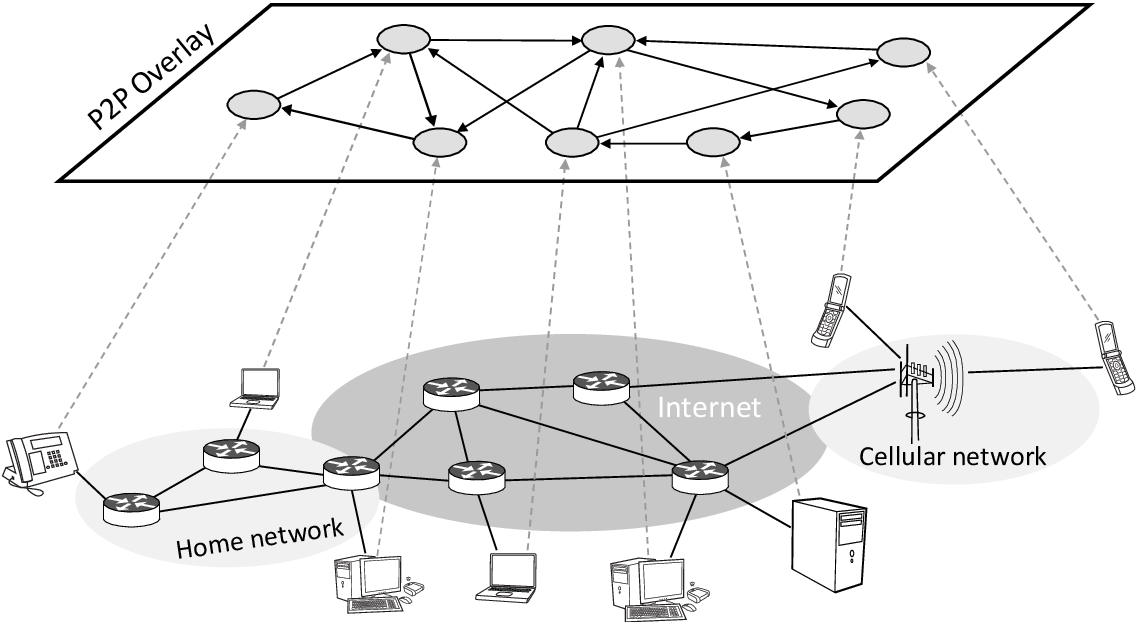
\includegraphics[width=0.9\linewidth]{images/overlay_network.png}
    \captionof{figure}{Peer-to-Peer-Overlay-Netzwerk mit darunterliegendem physischen Netzwerk \parencite{Kunzmann_OverlayNetworksImageSource}}
    \label{overlay_network}
\end{center}

\noindent In diesem Fall ist das physische Netzwerk das Internet. Das Overlay-Netzwerk ist eine logische Struktur, die es ermöglicht, die Kommunikation zwischen den Teilnehmern zu organisieren. Es besteht aus einer Reihe von Knoten, die über eine logische Verbindung miteinander verbunden sind. Die Verbindungen zwischen den Knoten werden durch Routing-Algorithmen verwaltet \parencite{Lua_P2POverlayNetworksPaper}.

Beispiele für Routing-Algorithmen sind \textit{Kademlia}, \textit{Chord} und \textit{Pastry}. Diese drei Algorithmen verwenden sogenannte \textit{Distributed Hash Tables}, um die Knoten zu verwalten. \textit{Distributed Hash Tables} (kurz: DHTs) sind verteilte Datenstrukturen, die in Peer-to-Peer-Netzwerken verwendet werden, um effizient Schlüssel-Wert-Paare zu speichern und abzurufen. Anders als herkömmliche zentralisierte Datenbanken oder Speicherlösungen benötigen DHTs keinen zentralen Server zur Speicherung oder Verwaltung von Daten. Sie funktionieren auf Basis von Hash-Funktionen, die einen Schlüssel in einen eindeutigen Hash umwandeln. Diese Hashes dienen als Adressen, um zu bestimmen, wo die entsprechenden Daten im Netzwerk gespeichert sind. Die Daten werden über verschiedene Peers im Netzwerk verteilt, wobei jeder Peer nur einen Teil der Daten basierend auf seinem Verantwortungsbereich speichert . Um effizient auf die gespeicherten Daten zuzugreifen, verwenden DHTs  Routing-Algorithmen wie Pastry, Kademlia oder Chord. Diese Algorithmen ermöglichen es, Peers im Netzwerk zu finden, die für die Speicherung oder Abfrage von Daten zuständig sind, selbst wenn sich die Netzwerktopologie ständig verändert. Ein großer Vorteil von DHTs ist ihre Skalierbarkeit. Sie können mit der Netzwerkgröße wachsen, ohne an Effizienz zu verlieren. Neue Peers können nahtlos hinzugefügt werden, und die Struktur der DHT passt sich dynamisch an Veränderungen im Netzwerk an \parencite[S. 43-46]{Balakrishnan_LookingUpDataInP2PSystems} \parencite[postnote]{Stoica_Chord,Rowstron_Pastry,Maymounkov_Kademlia}.


\subsection{Kademlia vs. Chord vs. Pastry}

\textit{Kademlia} ist ein Peer-to-Peer-Protokoll, das für die Organisation von Knoten in einem Netzwerk verwendet wird. Es ist ein strukturiertes Peer-to-Peer-Netzwerk, das auf einer K-Bucket-Struktur basiert. Die K-Buckets enthalten eine Liste von Knoten für verschiedene Schlüsselbereiche basierend auf ihrer Nähe, die durch XOR-Distanzen der IDs berechnet wird. Die Verbindungen zwischen den Knoten sind asymmetrisch, und jeder Knoten speichert Informationen über andere Knoten in seinen K-Buckets. Bei der Suche nach einem bestimmten Schlüssel erfolgt das Routing durch die XOR-Entfernung, wodurch die nächsten Knoten für diesen Schlüssel gefunden werden. Dieses Verfahren ermöglicht eine logarithmische Anzahl von Schritten für die Suche und bietet eine robuste Struktur, die gut mit dynamischen Netzwerkänderungen umgehen kann \parencite[S. 1-2]{Maymounkov_Kademlia}.

\textit{Chord} ist ein weiteres Peer-to-Peer-Protokoll, das für die Organisation von Knoten in einem Netzwerk verwendet wird. Es ist ebenfalls ein strukturiertes Peer-to-Peer-Netzwerk, basiert allerdings auf einer Ringstruktur. Die Knoten sind in einem Ring angeordnet und jeder Knoten ist für einen bestimmten Schlüsselbereich verantwortlich. Die Verbindungen zwischen den Knoten sind durch ihren Platz im Ring definiert, wobei jeder Knoten eine Verbindung zu seinem nächsten Nachbarn im Uhrzeigersinn hat. Bei der Suche nach einem bestimmten Schlüssel durchläuft eine Anfrage einen logarithmischen Pfad im Ring, wobei die Knoten auf dem Weg begrenzte Informationen über andere Knoten behalten, um Anfragen weiterzuleiten. Dieses Modell ist recht einfach und effizient für viele Anwendungsfälle, aber es könnte anfällig sein für Engpässe oder längere Suchzeiten, insbesondere wenn das Netzwerk dynamisch ist und sich die Konfiguration häufig ändert \parencite[S. 1-2]{Stoica_Chord}.

Auch \textit{Pastry} basiert auf einer Ringstruktur und ist darauf ausgerichtet, die Übertragung von Daten und die Suche nach Peers in großen, dynamischen Netzwerken zu optimieren. Im Kern funktioniert Pastry wie folgt: Es organisiert Peers in einem virtuellen Ring, wobei jeder Peer eine eindeutige ID hat. Diese IDs sind im metrischen Raum angeordnet, wodurch ähnliche IDs oder Schlüssel ähnliche Peers im Ring finden. Jeder Peer in Pastry verfügt über Routing-Tabellen, die Informationen über andere Peers im Ring enthalten, die in der Nähe ihrer eigenen ID liegen. Diese Routing-Tabellen ermöglichen es, Peers in logarithmischer Zeit zu erreichen, unabhängig von der Netzwerkgröße. Wenn eine Nachricht gesendet werden soll, wählt der Sender anhand der Ziel-ID des Peers den nächsten Peer in seiner Routing-Tabelle aus, der der Ziel-ID am nächsten liegt. Diese Prozedur wird iterativ wiederholt, bis die Nachricht ihren Ziel-Peer erreicht hat. Pastry ist widerstandsfähig gegen Ausfälle und kann sich an dynamische Netzwerkänderungen anpassen, indem es die Routing-Struktur und -Tabellen entsprechend aktualisiert \parencite[S. 331-339]{Rowstron_Pastry}.


Für den Anwendungsfall des Instant Messaging ist die effektive Bewältigung von \textit{Churn} von entscheidender Bedeutung. Churn bezieht sich auf die häufigen Ein- und Austritte von Teilnehmern in einem Peer-to-Peer-Netzwerk. In einem Instant Messaging Kontext bedeutet dies, dass Benutzer sich ständig anmelden oder abmelden. Ein Protokoll, das gut mit Churn umgehen kann, ist entscheidend, um eine zuverlässige und nahtlose Kommunikation zu gewährleisten. Das richtige Handling von Churn ist daher ein Schlüsselfaktor für die Leistungsfähigkeit und Stabilität eines Instant Messaging Protokolls \parencite[S. 316-317]{Peris_KademliaChurn}.

Kademlia ist bekannt für seine Effizienz bei der Skalierung und der Robustheit gegenüber Churn. Es verwendet eine XOR-Metrik, um Peers in einem logarithmischen Adressraum zu organisieren, was zu kurzen Pfaden für Anfragen führt. Dadurch eignet es sich gut für große, dynamische Netzwerke, da es leicht neue Peers integrieren und Ausfälle tolerieren kann \Parencite{MedranoChavez_ChordKademliaHighChurnScenarios}.

Chord hingegen basiert, wie bereits angesprochen, auf einem ringförmigen Adressraum, in dem jeder Peer für eine bestimmte Adresse verantwortlich ist. Es bietet eine deterministische Routing-Tabelle und erfordert im Vergleich zu Kademlia weniger Overhead für Routinginformationen. Dies macht Chord gut geeignet für statischere Netzwerke, in denen die Stabilität der Routinginformationen wichtiger ist als die Anpassungsfähigkeit an dynamische Veränderungen \parencite{Stoica_Chord}.

Pastry verwendet eine gemeinsame Präfix-Länge als Grundlage für die Adressierung und organisiert Peers in einem eindimensionalen Raum. Es bietet eine gute Balance zwischen Effizienz und Skalierbarkeit, indem es kurze Routingpfade mit geringem Overhead ermöglicht. Pastry eignet sich gut für mittelgroße Netzwerke mit moderater Dynamik und bietet eine solide Leistung bei der Bewältigung von Knotenausfällen \parencite{Rowstron_Pastry}.

Insgesamt bieten alle drei Algorithmen Lösungen für verteilte Systeme, variierend in ihrer Anpassungsfähigkeit, Skalierbarkeit und Effizienz je nach den spezifischen Anforderungen des Netzwerks. Die Wahl zwischen Kademlia, Chord und Pastry hängt von Faktoren wie der Größe des Netzwerks, der erwarteten Dynamik (Churn) und der Priorität zwischen Skalierbarkeit und Routingstabilität ab.

\subsection{Angriffe auf Peer-to-Peer-Netzwerke}

\subsubsection{Denial-of-Service-Angriff}

Mit einem \textit{Denial-of-Service}-Angriff (kurz: \textit{DoS-Angriff}) wird versucht, die Verfügbarkeit eines Dienstes zu beeinträchtigen, indem die Ressourcen des Dienstes erschöpft werden, sodass diese ausfallen \parencite{Bicakci_DoSAttacks}. In einem Peer-to-Peer-Netzwerk kann ein DoS-Angriff auf verschiedene Arten durchgeführt werden. Eine Möglichkeit ist es, einen Peer mit Anfragen zu überfluten, um ihn zu überlasten. Eine andere Möglichkeit ist es, einen Peer mit gefälschten Informationen zu überfluten, um ihn zu täuschen. Beide Methoden führen dazu, dass der Peer nicht mehr in der Lage ist, seine Aufgaben zu erfüllen, was zu einem Ausfall des Dienstes führt. Dieser Angriff wird noch effektiver, wenn er von mehreren Angreifern gleichzeitig durchgeführt wird. Dies wird als \textit{Distributed Denial-of-Service}-Angriff (kurz: \textit{DDoS-Angriff}) bezeichnet. Bei einem DDoS-Angriff wird der Peer mit Anfragen von mehreren Angreifern überflutet, was es schwieriger macht, den Angriff zu stoppen \Parencite[S. 6]{Baptiste_AttacksOnP2PNetworks}.


\subsubsection{Sybil-Angriff}
\label{subsubsec:sybil_attack_p2p}

Der Sybil-Angriff ist nicht spezifisch für Blockchain, sondern kann in jedem Peer-to-Peer-Netzwerk durchgeführt werden. Bei diesem Angriff erstellt ein einzelner Angreifer mehrere Identitäten, um die Kontrolle über das Netzwerk zu erlangen. Der Angreifer kann dann die Kontrolle über das Netzwerk übernehmen, indem er die Mehrheit der Identitäten kontrolliert \parencite[S. 251]{Douceur_SybilAttack}. Nach einer erfolgreichen Übernahme von Teilen des Netzwerks, besteht die Möglichkeit der Durchführung eines \textit{Eclipse}-Angriffs, welcher im nächsten Abschnitt erklärt wird \parencite[S. 13-15]{Baptiste_AttacksOnP2PNetworks}.


\subsubsection{Eclipse-Angriff}
\label{subsubsec:eclipse_attack_p2p}

Bei einem \textit{Eclipse}-Angriff wird versucht, einen Peer von allen anderen Peers im Netzwerk zu isolieren. Dies wird erreicht, indem bereits durch den vorhergegangenen Sybil-Angriff die Mehrheit der Peers kontrolliert wird. Der Angreifer kann dann die Verbindungen des Opfers zu anderen Peers im Netzwerk verhindern, indem er die Verbindungen zu anderen Peers kontrolliert \Parencite[S. 14]{Baptiste_AttacksOnP2PNetworks}. 



\section{Sicherheit}
\label{sec:sicherheit_basics}

Wie aus der Abbildung in Abschnitt \ref{subsec:overlay_netzwerke} \textit{\nameref{subsec:overlay_netzwerke}} ersichtlich ist, ist das Overlay-Netzwerk die oberste Schicht des Peer-to-Peer-Netzwerks. Es sorgt dafür, dass sich die Teilnehmer des Netzwerks finden können. Die eigentliche Kommunikation, also das Senden und Empfangen von Nachrichten, erfolgt jedoch über das Internet. Da das Internet ein öffentliches Netzwerk ist, besteht die Gefahr, dass die Nachrichten abgefangen und mitgelesen werden können. Die Nachrichten müssen über Verteilerknoten oder Access Points übertragen werden, die nicht vertrauenswürdig sind. Um ein Mitlesen oder Verändern der Nachrichten zu verhindern, muss die Kommunikation abgesichert werden. 

Mittels Kryptografie kann die Vertraulichkeit, Integrität und Authentizität der Kommunikation gewährleistet werden \Parencite[S. 7]{Hellmann_IT-Sicherheit}.


\subsection{Vertraulichkeit}
\label{subsec:vertraulichkeit_basics}

Die Vertraulichkeit der Kommunikation wird durch Verschlüsselung gewährleistet. Man unterschiedet zwei Formen der Kryptografie: \textit{symmetrische} und \textit{asymmetrische} Kryptografie. Bei der \textit{symmetrischen} Kryptografie wird ein und derselbe Schlüssel zum Verschlüsseln und Entschlüsseln der Nachricht verwendet. Der Sender der Nachricht verschlüsselt die Nachricht mit einem Schlüssel und sendet die nun verschlüsselte Nachricht an den Empfänger. Der Empfänger kann die Nachricht mit dem gleichen Schlüssel entschlüsseln. Dadurch kann ein Angreifer, der die Nachricht abfängt, diese nicht entschlüsseln, da er den Schlüssel nicht kennt. Abbildung \ref{fig:symmetrische_verschluesselung} zeigt den Ablauf der symmetrischen Verschlüsselung.

\begin{center}
    \captionsetup{type=figure}
    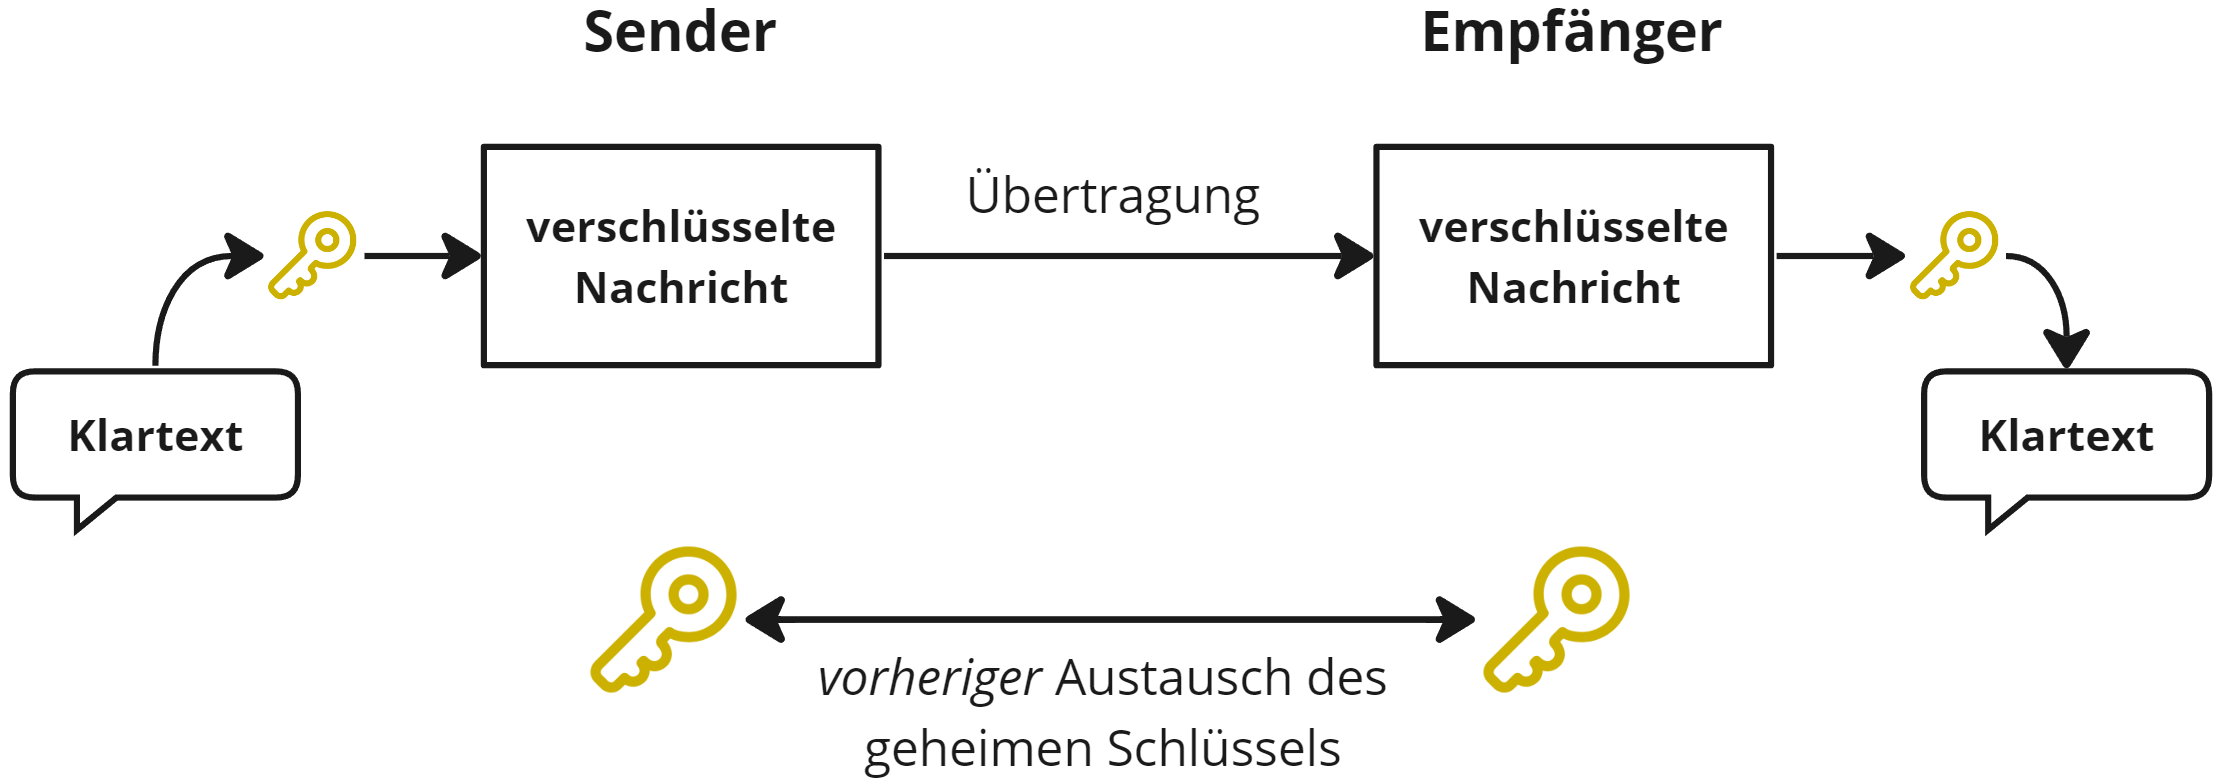
\includegraphics[width=1\linewidth]{images/symmetric_encryption.png}
    \caption{Symmetrische Verschlüsselung (in Anlehnung an \cite{ElektronikKompendium_symmetrischeVerschluesselung})}
    \label{fig:symmetrische_verschluesselung}
\end{center}

\noindent Das Problem bei der symmetrischen Kryptografie ist, dass der Schlüssel zu Beginn der Kommunikation vom Sender an den Empfänger gelangen muss. Dies stellt eine Herausforderung dar, wenn Sender und Empfänger sich noch nicht kennen und noch nie zuvor miteinander kommuniziert haben oder noch nicht über andere Wege einen Schlüssel ausgetauscht haben. Sollte der Schlüssel bei der Übertragung über einen unsicheren Kanal abgefangen werden, kann der Angreifer die Kommunikation entschlüsseln und somit mitlesen \Parencites[S. 644]{DiffieHellman_NewDirectionsInCryptography}[S. 5-8]{Wong_KryptoPraxis}. 

In diesem Fall kann eine Schlüsselvereinbarung verwendet werden, um einen gemeinsamen Schlüssel zu erhalten. Bei der Schlüsselvereinbarung wird ein Schlüssel zwischen zwei Parteien vereinbart, ohne dass dieser über einen unsicheren Kanal übertragen werden muss \Parencite[S. 102]{Wong_KryptoPraxis}. Abbildung \ref{fig:schluesselvereinbarung} zeigt den Ablauf der Schlüsselvereinbarung.

\begin{center}
    \captionsetup{type=figure}
    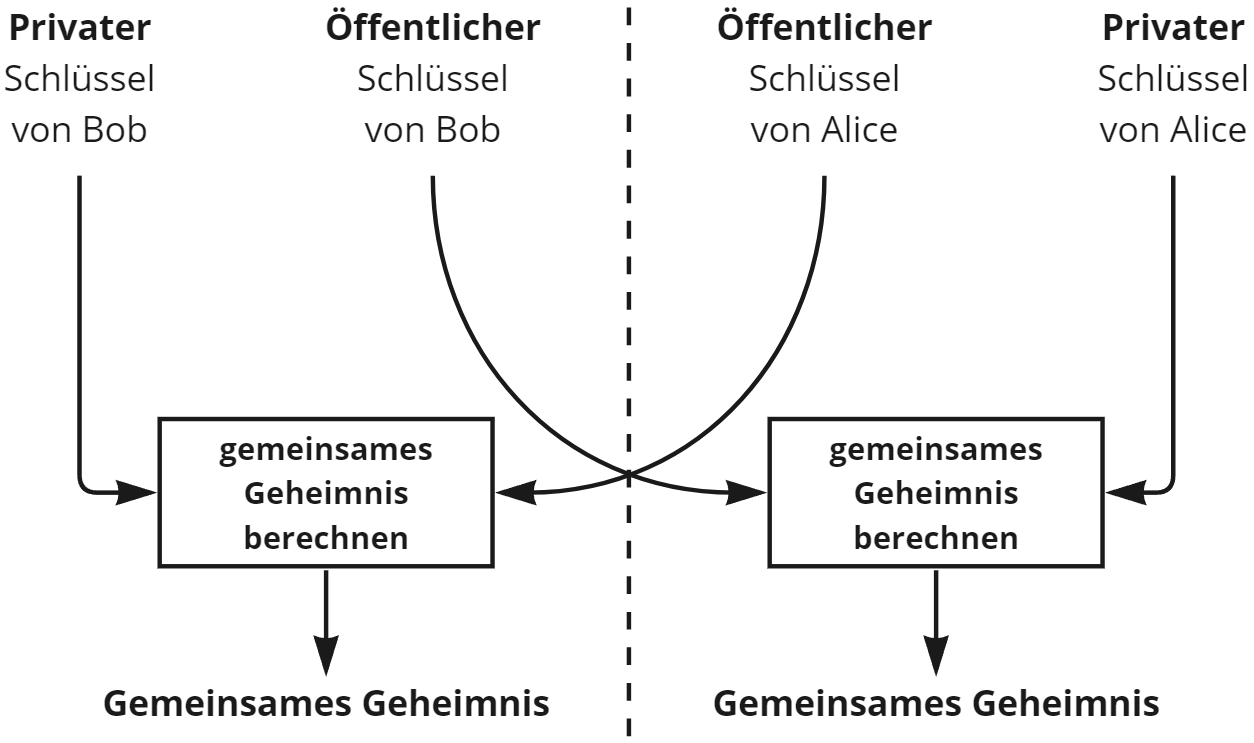
\includegraphics[width=0.7\linewidth]{images/key_exchange.png}
    \caption{Schlüsselvereinbarung (in Anlehnung an \cite[S. 102]{Wong_KryptoPraxis})}
    \label{fig:schluesselvereinbarung}
\end{center}

\noindent Beide Teilnehmer generieren einen privaten Schlüssel und einen öffentlichen Schlüssel. Durch die Kombination des öffentlichen Schlüssels des anderen Teilnehmers und des eigenen privaten Schlüssels wird ein gemeinsames Geheimnis berechnet. Dieses gemeinsame Geheimnis kann dann für die symmetrische Verschlüsselung verwendet werden, da dadurch beide Teilnehmer den gleichen Schlüssel besitzen \Parencite[S. 102]{Wong_KryptoPraxis}.


Bei der \textit{asymmetrische} Kryptografie (auch \textit{Public-Key-Kryptografie} genannt) wird anstatt nur eines Schlüssels ein Schlüsselpaar generiert, das aus einem öffentlichen und einem privaten Schlüssel besteht. Der öffentliche Schlüssel des Empfängers wird zum Verschlüsseln der Nachrichten verwendet und zum Entschlüsseln der Nachrichten wird der private Schlüssel des Empfängers verwendet. Der öffentliche Schlüssel des Empfängers kann von jedem verwendet werden, um Nachrichten an den Empfänger zu verschlüsseln. Nur der Empfänger kann die Nachrichten entschlüsseln, da nur er den privaten Schlüssel besitzt. Der Ablauf der asymmetrischen Verschlüsselung ist in Abbildung \ref{fig:asymmetrische_verschluesselung} dargestellt.


\begin{center}
    \captionsetup{type=figure}
    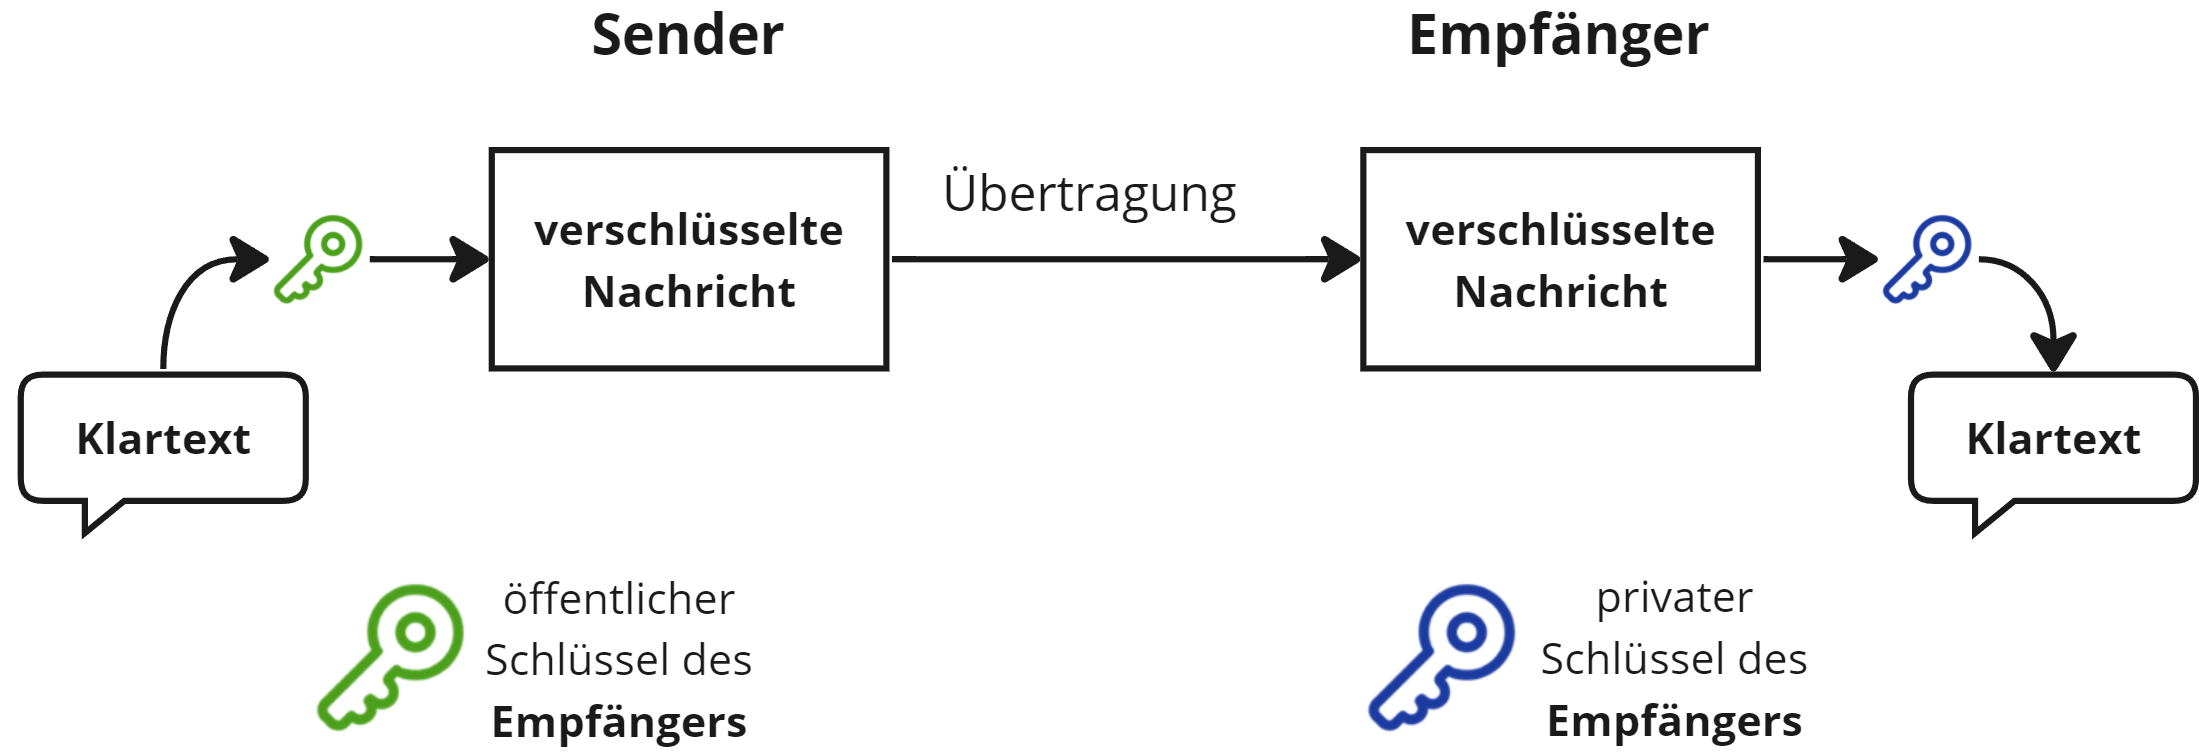
\includegraphics[width=1\linewidth]{images/asymmetric_encryption.png}
    \caption{Asymmetrische Verschlüsselung (in Anlehnung an \cite{ElektronikKompendium_asymmetrischeVerschluesselung})}
    \label{fig:asymmetrische_verschluesselung}
\end{center}

\noindent Es ist außerdem nicht möglich, Nachrichten, die mit dem öffentlichen Schlüssel verschlüsselt wurden, mit diesem auch wieder zu entschlüsseln \parencite{ElektronikKompendium_asymmetrischeVerschluesselung}. 

Diese kryptografische Verfahren können kombiniert werden, um die Vorteile von diesen zu nutzen. Der Schlüsselaustausch wird mit der asymmetrischen Verschlüsselung durchgeführt und die eigentliche Kommunikation wird mit der symmetrischen Verschlüsselung durchgeführt.


\subsection{Integrität}
\label{subsec:integritaet_signatur}

Um die Integrität der Kommunikation zu gewährleisten, wird Hashing verwendet. Das Hashing von Daten erfordert die Verwendung einer \textit{Hash-Funktion}. Hash-Funktionen sind Funktionen, die eine Eingabe beliebiger Länge in eine Ausgabe fester Länge umwandeln. Dabei ist es wichtig, dass die Hash-Funktion zwei Eigenschaften erfüllt: \textit{Einwegfunktion} und \textit{Kollisionsresistenz}. Eine Hash-Funktion erfüllt die Eigenschaft der Einwegfunktion, wenn es nicht möglich ist, von der Ausgabe auf die Eingabe zu schließen. Das bedeutet, dass es nicht möglich ist, aus dem Hash-Wert die ursprünglichen Daten zu rekonstruieren. Die Eigenschaft der Kollisionsresistenz ist erfüllt, wenn es nicht möglich ist, zwei verschiedene Eingaben zu finden, die auf den gleichen Hash-Wert abgebildet werden \parencites[S. 12-13]{Brünnler_BlockchainKurzGut}[S. 6]{Fill_BlockchainGrundlagen}.

Das Ergebnis der Hash-Funktion ist eine Zeichenkette, die aus einer festen Anzahl an Zeichen besteht und als \textit{Hash-Wert} oder auch nur \textit{Hash} bezeichnet wird. Der Hash-Wert ist ein eindeutiger Fingerabdruck der Daten, die in die Hash-Funktion eingegeben wurden. Sollte sich also der Inhalt der Daten ändern, ändert sich auch der Hash-Wert. 


\subsection{Authentizität}

In Kombination mit einer sogenannten Signatur kann zusätzlich zur Integrität auch die Authentizität einer Nachricht gewährleistet werden. Abbildung \ref{fig:signatur} zeigt, wie eine Nachricht digital signiert wird.

\begin{center}
    \captionsetup{type=figure}
    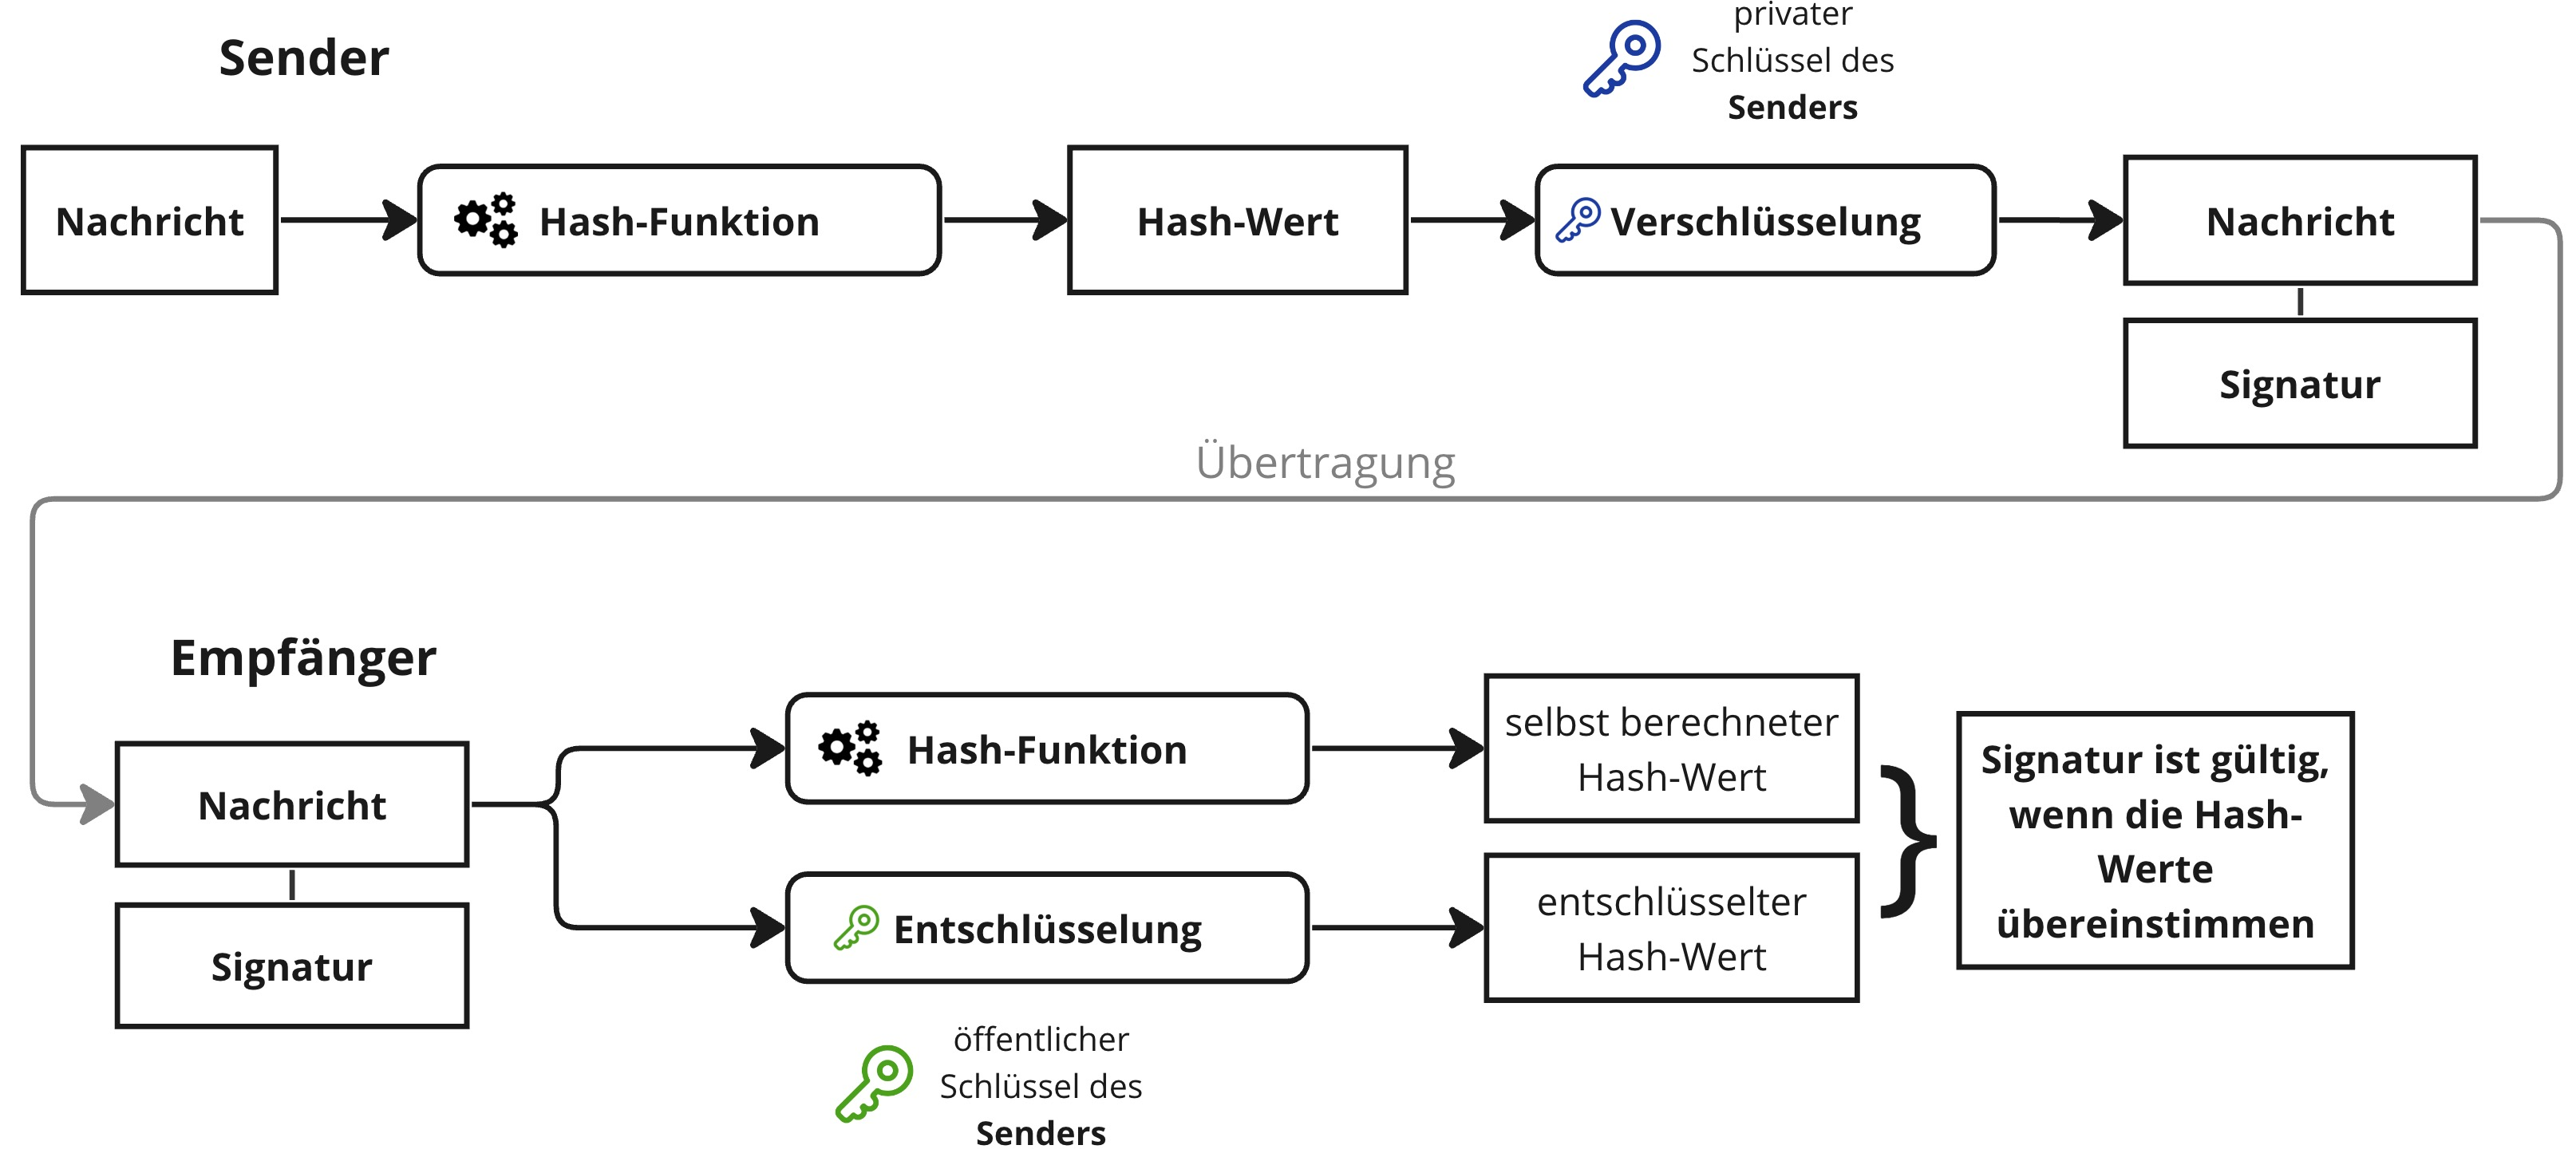
\includegraphics[width=1\linewidth]{images/signatur_2.jpg}
    \caption{Signieren einer Nachricht (in Anlehnung an \cite{DocuSign_digitaleSignaturen})}
    \label{fig:signatur}
\end{center}


\noindent Der Sender berechnet den Hash-Wert der Nachricht, verschlüsselt diesen mit seinem privaten Schlüssel. Das Ergebnis ist die digitale Signatur, welche an die Nachricht angehängt wird. Der Empfänger braucht den öffentlichen Schlüssel des Senders, um die Signatur zu entschlüsseln. Dafür gibt es verschiedene Möglichkeiten. Eine Möglichkeit ist, dass der Sender den öffentlichen Schlüssel dem Empfänger vorher über einen sicheren Kanal übermittelt. Eine andere Möglichkeit ist, dass der öffentliche Schlüssel des Senders in einem öffentlichen Schlüsselverzeichnis gespeichert ist. Wenn der Empfänger den öffentlichen Schlüssel des Senders besitzt, kann er die Signatur entschlüsseln. Gleichzeitig berechnet der Empfänger den Hash-Wert der Nachricht. Wenn der berechnete Hash-Wert mit dem entschlüsselten Hash-Wert übereinstimmt, kann der Empfänger einerseits sicher sein, dass die Nachricht nicht verändert wurde und somit die Integrität der Nachricht gewährleistet ist und andererseits, dass die Nachricht vom Sender stammt und somit die Authentizität der Nachricht gewährleistet ist. Falls der berechnete Hash-Wert nicht mit dem entschlüsselten Hash-Wert übereinstimmt, wurde die Nachricht entweder verändert oder die Nachricht stammt nicht vom erwarteten Sender \Parencite[S. 73-78]{Hellmann_IT-Sicherheit}.


\subsection{Ende-zu-Ende-Verschlüsselung}
\label{subsec:signal_protokoll_basics}

% Was ist Ende-zu-Ende-Verschlüsselung? Wie entsteht diese? Warum zeige ich das anhand des Signal-Protokolls?

Die behandelten Sicherheitsmechanismen können zu einer sogenannten Ende-zu-Ende-Verschlüsselung kombiniert werden. Diese erlaubt es, dass nur der Sender und der Empfänger die Nachrichten lesen können. Eine moderne Variante der Ende-zu-Ende-Verschlüs-\\selung ist das Signal-Protokoll. Dies wird auch in der Signal-App verwendet (\ref{subsubsection:signal} \textit{\nameref{subsubsection:signal}}). Im Folgenden wird das Signal-Protokoll genauer beschrieben.

Zu Beginn einer Sitzung wird ein gemeinsamer Schlüssel zwischen den Teilnehmern vereinbart. Das Signal-Protokoll verwendet hierfür ein spezielles Verfahren, das sich \textit{Extended Triple Diffie-Hellman} oder auch kurz \textit{X3DH} nennt. Dieses kombiniert mehrere Schlüsselaustauschaktionen, und ist dadurch in der Lage, einen gemeinsamen Schlüssel zu berechnen, ohne dass der Kommunikationspartner direkt erreichbar sein muss. Dazu werden mehrere flüchtige Schlüssel auf einem Server gespeichert. Dies dient dazu, dass eine Kompromittierung dieser Schlüssel nicht die Sicherheit der Kommunikation gefährdet, da diese nur für eine begrenzte Zeit gültig sind und für jede Sitzung neu generiert werden \Parencite[S. 249-252]{Wong_KryptoPraxis}.


Da solch eine Sitzung sehr lange dauern kann, generiert das Signal-Protokoll auch für jede Nachricht einen neuen Schlüssel. Hierfür wird der sogenannte \textit{Double Ratchet Algorithmus} verwendet. Dieser bildet den Kern des Signal-Protokolls. Eine \textit{Ratchet} (zu Deutsch: \textit{Ratsche}) ist ein Werkzeug, das nur in eine Richtung gedreht werden kann. Diese Eigenschaft wird auf die verwendeten Schlüssel angewendet. Dadurch ist es nicht möglich, vorherige Schlüssel zu berechnen, was auch als \textit{Forward Secrecy} bezeichnet wird. Der Algorithmus verwendet zwei Ratchet-Schritte. Der erste Ratchet-Schritt verwendet einen symmetrischen Schlüssel. Basierend auf dem vorher, durch X3DH vereinbarten, gemeinsamen Schlüssel, generieren die Kommunikationspartner jeweils einen Empfangs- und einen Sendeschlüssel. Jede gesendete Nachricht wird dem Sendeschlüssel verschlüsselt und jede empfangene Nachricht wird mit dem Empfangsschlüssel entschlüsselt. Nach jeder Nachricht werden die Schlüssel durch eine Schlüsselableitungsfunktion aktualisiert. Der zweite Ratchet-Schritt ist ein asymmetrischer Schlüsselaustausch, den die Kommunikationspartner periodisch austauschen \Parencite[S. 252-257]{Wong_KryptoPraxis}. 

Vereinfacht kann der Double Ratchet Algorithmus für einen der Kommunikationspartner folgendermaßen dargestellt werden (siehe Abbildung \ref{fig:double_ratchet}):


\begin{center}
    \captionsetup{type=figure}
    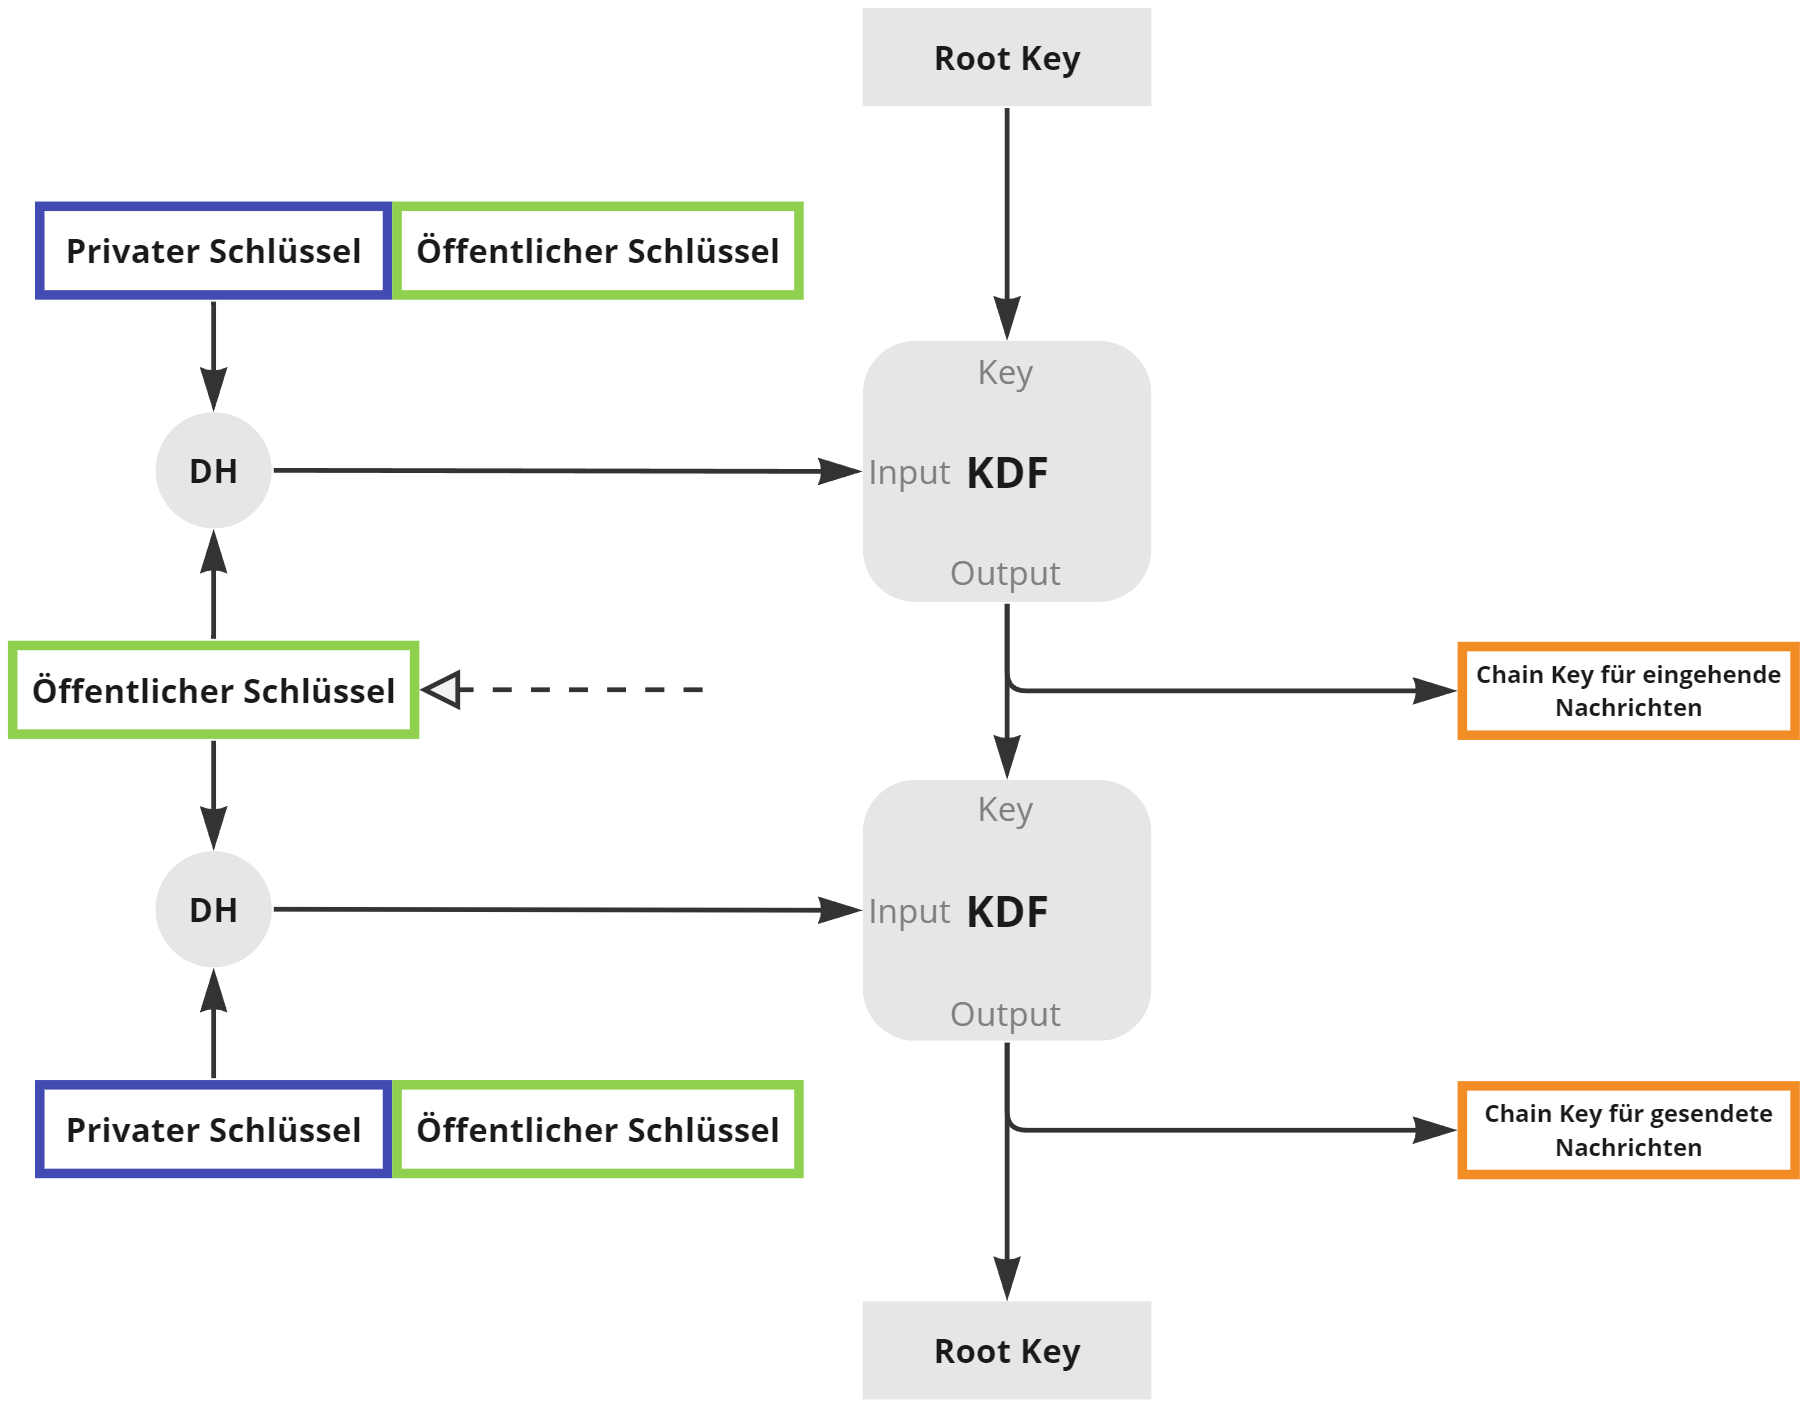
\includegraphics[width=0.8\linewidth]{images/double_ratchet_altered.png}
    \caption{Vereinfachter Double Ratchet Algorithmus (in Anlehnung an \cite{Signal_DoubleRatchet})}
    \label{fig:double_ratchet}
\end{center}

\noindent Links ist der zweite Ratchet-Schritt zu sehen (asymmetrischer Schlüsselaustausch). In der Abbildung ist dieser mit \textit{DH} gekennzeichnet, was für den Diffie-Hellman-Schlüsselaus-\\tausch steht. Auf der rechten Seite befindet sich der erste Ratchet-Schritt. Die Schlüsselableitungsfunktion wird in der Abbildung mit \textit{KDF} bezeichnet. Aus dieser werden die symmetrischen Schlüssel (in der Abbildung als \textit{Chain Key} bezeichnet) abgeleitet, die die jeweiligen Nachrichten ver- und entschlüsseln.



\section{Blockchain-Technologie}
Die Blockchain-Technologie ist... . Blockchains sind auch bekannt als Distributed Ledger 
Technology (DLT) und das sind auch nur verteilte Datenbanken. Die Blockchain ist eine
spezielle Form der DLT. Die Blockchain ist eine Kette von Blöcken, die jeweils einen
Hash des vorherigen Blocks enthalten. Die Blockchain ist eine dezentrale Datenbank, die
von allen Teilnehmern des Netzwerks verwaltet wird.

Proof of Work und Proof of Stake sind zwei verschiedene Konsensmechanismen, die verwendet
werden, um die Blockchain zu validieren. Proof of Work ist der Konsensmechanismus, der
von Bitcoin verwendet wird. Proof of Stake ist der Konsensmechanismus, der von Ethereum (2.0)
verwendet wird.

\subsection{Ethereum}
\label{sec:ethereum_basics}

Ethereum ist eine der führenden Blockchain-Plattformen und wurde 2015 von Vitalik Buterin, Gavin Wood und anderen entwickelt. Im Gegensatz zu Bitcoin, das hauptsächlich als digitale Währung fungiert, ermöglicht Ethereum die Ausführung von Smart Contracts und die Entwicklung von dezentralen Anwendungen (engl. \textit{decentralized Applications}, kurz \textit{DApps}) \Parencites[S. 720]{Sorge_BitcoinZahlungsmittelDerZukunft}[S. 1-2]{Perez_SmartContractVulnerabilities}. Bis 2022 wurde als Konsensmechanismus Proof-of-Work verwendet, der jedoch 2022 durch Proof-of-Stake ersetzt wurde. Seitdem existieren zwei Versionen von Ethereum: \textit{Ethereum Classic} und \textit{Ethereum 2.0}. Ethereum Classic verwendet Proof-of-Work, während Ethereum 2.0 Proof-of-Stake verwendet \Parencite{EthereumClassic_ResearcherFAQs}.

Ether (ETH) ist die native Kryptowährung von Ethereum und wird für Transaktionen innerhalb des Netzwerks verwendet. Es dient auch als Anreiz für diejenigen, die an der Sicherung des Netzwerks durch Mining (bei PoW) oder Validierung (bei PoS) von Transaktionen beteiligt sind \parencite[S. 320-321]{Antonopoulos_MasteringEthereum}. Die Flexibilität von Ethereum und seine Fähigkeit, innovative Lösungen zu unterstützen, haben es zu einer der wichtigsten Plattformen in der Blockchain-Welt gemacht.

\subsection{Smart Contracts}
\label{subsection:smart_contracts}
% Smart Contracts werden per RPC aufgerufen.


Ein Smart Contract (zu Deutsch: \textit{intelligenter Vertrag}) ist im Grunde genommen ein selbstausführender Vertrag, der automatisch Aktionen auslöst, wenn bestimmte Bedingungen erfüllt sind \Parencite[S. 1-2]{Perez_SmartContractVulnerabilities}. Die Bezeichnung \textit{Smart Contract} ist eigentlich eine Fehlbezeichnung, da es sich weder um einen Vertrag im rechtlichen Sinne, noch um einen \textit{intelligenten} Vertrag handelt, doch der Begriff hat sich in der Blockchain-Community etabliert und wird deshalb weiterhin verwendet. Ein Lesezugriff auf einen Smart Contract ist kostenlos, ein Schreibzugriff hingegen kostet Geld, da die Transaktion in der Blockchain gespeichert werden muss. Dieses Geld wird als \textit{Gas} bezeichnet und ist eine Art Gebühr, die gezahlt werden muss, um die Rechenleistung des Netzwerks zu nutzen \Parencite[S. 127]{Antonopoulos_MasteringEthereum}. Um Gas zu erhalten, muss der Nutzer Ether eintauschen, die Währung der Ethereum-Blockchain.
Für das Protokoll dieser Arbeit wurden sowohl Lese- als auch Schreibzugriffe auf Smart Contracts implementiert (siehe Kapitel \ref{chap:entwurf_und_architektur} \textit{\nameref{chap:entwurf_und_architektur}}).

Die Plattform verwendet die objektorientierte Programmiersprache \textit{Solidity}, die speziell für Smart Contracts entwickelt wurde und stark an JavaScript angelehnt ist. Entwickler können mithilfe von Solidity Smart Contracts erstellen, die dann in der Ethereum-Blockchain ausgeführt werden und von jedem Teilnehmer des Netzwerks aufgerufen werden können \Parencite[S. 127-133]{Antonopoulos_MasteringEthereum}.

